With the $S$-matrix calculus and SASA we can fully describe stacks of homogeneous isotropic materials but we still have no understanding of what happens when we add a metasurface to a stack. To build some intuition for how a specific metasurface will affect the transmission spectrum of a stack we will need a little more theory on optics in materials. All optical properties of a material a captured by the $\vb D$ and $\vb H$ fields and in our context

\begin{equation}
    \vb D = 
    \epsilon_0 \, \vb E + \vb P =
    \epsilon_0\, \underbrace{\qty(1 + \chi)}_{
         := \epsilon
    }\, \vb E
\end{equation}

so the $\vb D$ field is determined by the $\vb E$ field and dielectric function $\epsilon$. In the following sections we will discuss which materials have which kind of dielectric function and how we can use these to gain some intuition for the optical mechanisms in a metasurface.

\paragraph{Dielectric Function}~\\
In the simplest model we can describe electrons in a material as an ensemble of harmonic oscillators

\begin{equation} \label{eq:bg:lorentz}
    m \ddot{\vb x} + m \gamma \dot{\vb x} + m \omega_0^2 \vb x = -e \vb E
\end{equation}
\indent
$\vb x$ displacement, $m$ electron mass, $e$ electron charge, $\gamma$ dampening factor, $\omega_0$ resonance frequency 
and the macroscopic polarization $\vb P$ is directly caused by this displacement $\vb x$

\begin{equation}
    \vb P = - \rho e \vb x
\end{equation}
\indent
$\rho$ density of electrons

If we assume a harmonic time dependency $\vb E(t) = \vb E_0 e^{i \omega t}$ equation \eqref{eq:bg:lorentz} is solved by 

\begin{equation}
    \vb x(t) = \frac{e}{m(\omega^2 + i \gamma \omega - \omega_0^2)} \vb E(t)
\end{equation}

and this results in a $\vb D$ field

\begin{equation}
    \vb D = 
    \epsilon_0 \underbrace{ 
    \qty(1 - \frac{f}{\omega^2 + i \gamma \omega - \omega_0^2})
    }_{
        =\epsilon
    }
    \vb E
\end{equation}
\indent
$f = \rho e^2 / \epsilon_0 m$ oscillator strength

In a real material there are always multiple resonance frequencies $\omega_m$ but in a good approximation these do not influence each other and the total dielectric function can be obtained simply by summing over all $\omega_m$

\begin{equation}
    \epsilon(\omega) = 
    1 + \sum_m \frac{f_m}{\omega_m^2 - \omega_0^2 - i \gamma \omega}
\end{equation}

\begin{figure}[H]
    \floatbox[{
    \capbeside
    \thisfloatsetup{capbesideposition={right,top},capbesidewidth=7cm}}]{figure}[\FBwidth]
    {\caption{
        }
    \label{fig:al:same_spec}}
    {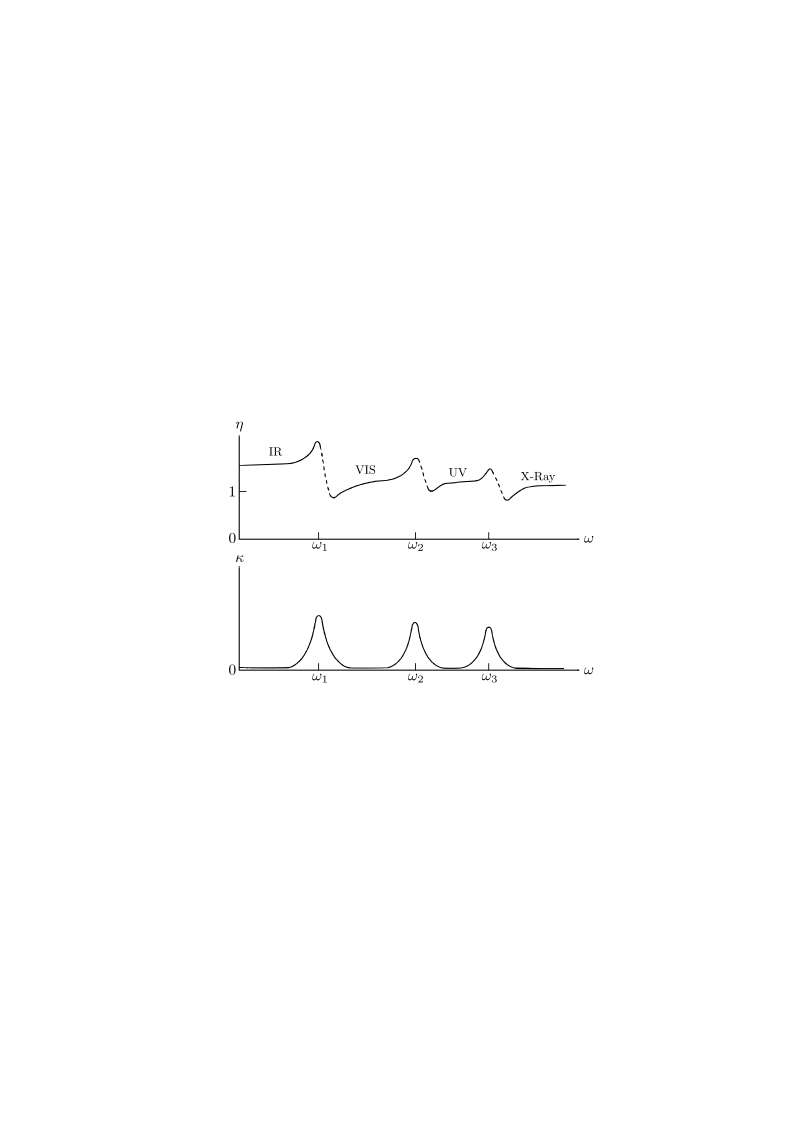
\includegraphics[width=0.55\textwidth]{bg_lorentz}}
\end{figure}